In the power calculations outlined above, the disease models are used to describe the distribution of the data under the alternative hypothesis.
Specifically, they are used to specify the conditional distributions of the allele variants, given the phenotypes.
The probability of observing a risk allele in the control group,
\begin{equation}
    f := \mathbb{P}[\,\text{risk allele}\,|\,\text{control group}\,] 
    = \frac{\mu_{21}}{1-\phi} 
    = \frac{\pi_{22} + \pi_{21}/2}{\pi_{22} + \pi_{21} + \pi_{20}},
\end{equation}
is fully determined by the disease model.
Similarly, the odds ratio between the two allele variants, 
\begin{equation}
    R:=\frac{\mu_{11}\mu_{22}}{\mu_{12}\mu_{21}} 
    = \frac{(\pi_{12} + \pi_{11}/2)(\pi_{20} + \pi_{21}/2)}{(\pi_{10} + \pi_{11}/2)(\pi_{22} + \pi_{21}/2)},
\end{equation}
is also determined by the disease model and its parameters.

In turn, the parameters $(f, R)$, together with the sample sizes $(\phi, n)$, fully describe the distribution of our data under the alternative hypothesis (by determining the probability vector $\mu$ and the sample size $n$).
Power of association tests, therefore, depends on (and only on) the set of ``canonical parameters'':

\begin{itemize}
    \item Risk allele frequency among the controls (f).
    \item Odds ratio (R) of having the defined trait between the two allele variants.
    \item One of the two equivalent ways of parametrizing the sample sizes.
\end{itemize}

We illustrates the common process of power analysis implemented in existing power calculators in Figure \ref{fig:flowchart}.

\begin{figure*}[!tpb]
    \centering
    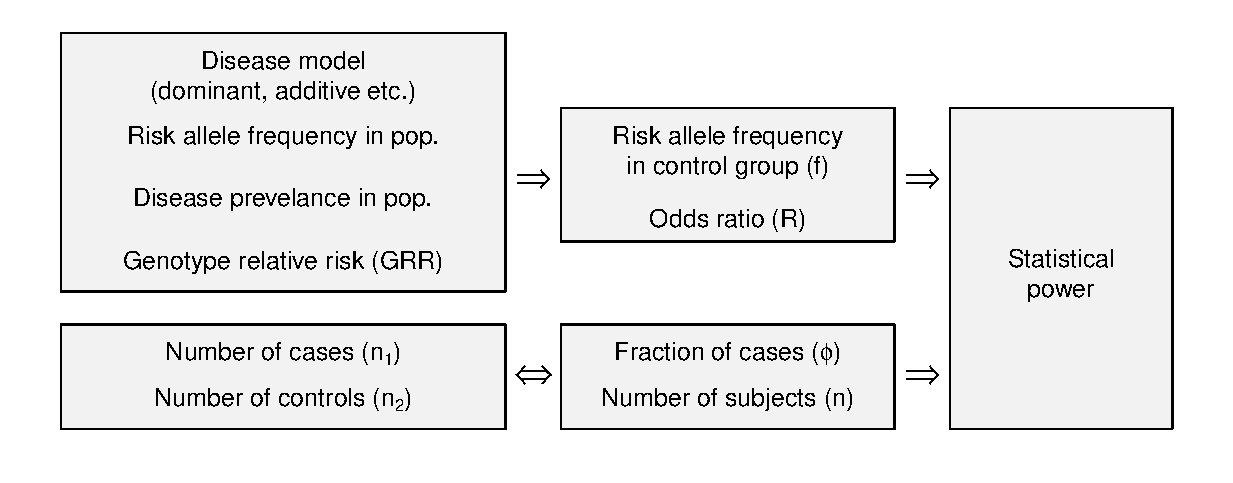
\includegraphics[width=\textwidth]{flowchart.eps}
    \caption{The process of a typical power analysis for genetic association tests.
    The quantities depend on, and can be calculated from the values of their parents in the directed graph. 
    Power can be calculated as long as one set of parameters in each branch is known.
    While there is a one-to-one correspondence between the sample size specifications $(n_1, n_2)$ and $(\phi, n)$, the mapping from disease model specifications to $(f, R)$ is many-to-one. 
    %That is, one cannot recover the disease model specifications from the allelic tables, or equivalently, reported risk allele frequencies and odds ratios.
    }
    \label{fig:flowchart}
\end{figure*}

Our discussion above shows that in power calculations, {\it we can either describe the alternative hypothesis with a disease model, or through the canonical parameters ($f, R$). Both approaches are sufficient for the purpose of power analysis.}

We remind readers that the risk allele frequency in the control group ($f$) is not equivalent to the risk allele frequency in the general population ($p$); odds ratio ($R$) is not equivalent to genotype relative risk (GRR).


\subsection{Conversion between the two specifications}

Notice that, as illustrated in  Figure \ref{fig:flowchart}, the power calculations are mediated through the canonical parameters, which are invariant to different model specifications.
That is, different disease model specifications may lead to the {\it same} set of canonical parameters ($f, R$), and consequently the) {\it same} distributions of the allele variant counts.
From a statistical perspective, the disease models that map to the same set of canonical parameters are equivalent in terms of power.

For example, the following set of disease models and parameters imply the same set of canonical parameters $(f = 0.290, R = 1.575)$, and therefore enjoy the same power at the same sample sizes ($n_1 = n_2 = 1000$).
\begin{center}
    \begin{tabular}{cc|cc}
    \hline
    Disease Model & $(\text{Prev}, p, \text{GRR})$ & $(f, R)$ & Power \\
    \hline 
    Multiplicative & $(0.1, 0.3, 1.500)$ & $(0.290, 1.575)$ & 0.990 \\
    Additive & $(0.1, 0.3, 1.588)$ & $(0.290, 1.575)$ & 0.990 \\
    Dominant & $(0.1, 0.3, 1.909)$ & $(0.290, 1.575)$ & 0.990 \\
    Recessive & $(0.1, 0.3, 2.666)$ & $(0.290, 1.575)$ & 0.990 \\
    \hline
    \end{tabular}
\end{center}

Conversely, different disease models with the same parameters, map to drastically different canonical parameters.
For example, the default disease model parameters in the GAS calculator,
\begin{align}
    \text{Disease prevalence in the population}: & \quad \text{Prev} = 0.1 \\
    \text{Risk allele frequency in the population}: & \quad p = 0.5\\
    \text{Genotype relative risk}: & \quad \text{GRR} = 1.5.
\end{align}
map to very different canonical parameters under different disease model assumptions (assuming the same sample sizes of $n_1 = n_2 = 1000$), which leads to drastically different statistical power.
\begin{center}
    \begin{tabular}{cc|cc}
    \hline
    Disease Model & $(\text{Prev}, p, \text{GRR})$ & $(f, R)$ & Power \\
    \hline 
    Multiplicative & $(0.1, 0.5, 1.5)$ & $(0.489, 1.568)$ & 0.995 \\
    Additive & $(0.1, 0.5, 1.5)$ & $(0.491, 1.453)$ & 0.920 \\
    Dominant & $(0.1, 0.5, 1.5)$ & $(0.495, 1.224)$ & 0.282 \\
    Recessive & $(0.1, 0.5, 1.5)$ & $(0.494, 1.281)$ & 0.098 \\
    \hline
    \end{tabular}
\end{center}

In the application, we provide users with a ``Disease model converter'' that implements this many-to-one conversion from the disease model specifications to the canonical parameters.


\subsection{Comparisons of the two approaches}
\label{subsec:comparing-two-approaches}

While the disease models may carry additional insights into the biological process, the canonical parameters also have their unique advantages.
We offer an incomplete list of comparisons of the two approaches, and discuss their usage in practice.

\subsubsection{Interpretability and communicability}

In general, geneticists and biostatisticians seem to agree that disease models are more interpretable.
The concept of genotype relative risks, in particular, seems easier to reason about than odds ratios in the canonical parameters definition.
Disease models also seem to be the de facto mode of model specification when performing power analysis for study planning and grant applications.

The ``nonparametric'' approach to model specification through the canonical parameters is somewhat lesser known to the statistical genetics community.
The canonical parameters are typically estimated and reported as outcomes of the research, but not used as inputs to the power analysis for planning purposes.

\subsubsection{Availability of parameter estimates}

The canonical parameters $f$ and $R$ can be estimated from data collected in the study.
They are also reported and curated in GWAS catalogs such as the NHGRI-EBI Catalog \citep{MacArthur16}.

On the other hand, accurate information regarding the disease model parameters can be more difficult to obtain, partly because some parameters in the disease models cannot be estimated from the association studies alone.

In particular, disease prevalence in population (Prev), as well as RAF in population ($p$), must be obtained from other studies or surveys targeting the general population; the association studies, unless matching the proportion of cases in the population vs in the study ($\phi=\text{Prev}$), cannot produce estimates without using external information.
Genetic association studies rarely explicitly estimate the disease model and its parameters.
In fact, we are not aware of a GWAS catalog that reports and curates the disease models and their estimated parameters.

This paucity of information on disease model parameters is not an issue if we are planning to study a trait for which we have little prior knowledge.
In this case, the purpose of power analysis is to determine the range of models and parameters that lead to discovery of associations, given the study designs.

In contrast, in confirmatory / follow-up studies and systematic reviews, our main interest is in the statistical validity of the reported findings.
Power analysis then serves to find efficient designs, and to validate the claims made.
Knowledge obtained in prior studies (in the form of parameter estimates) are indeed necessary.

\subsubsection{Robustness against model misspecification}

Disease models are useful in as much as they help us understand the biology behind the data we observe.
Unfortunately, like all models, they can be misspecified. 
For example, the following genotype relative risks,
\begin{equation*}
    \frac{\pi_{10}}{\pi_{10} + \pi_{20}} : \frac{\pi_{11}}{\pi_{11} + \pi_{21}} : \frac{\pi_{12}}{\pi_{12} + \pi_{22}}
    = 1 : 3 : 4,
\end{equation*}
does not follow any of the common disease models.
In this case, different studies may come up with different disease models (say, Dominant and Additive), and of course, different parameter estimates.

Suppose a researcher wishes to perform a meta analysis or confirmatory experiment of the existing results, where the literature reports inconsistent estimates of disease models and parameters,
he would a have a difficult time pooling the information from these different sources. 
And even when they are pooled, the resulting model usually does not fall in one of the familiar categories --- there is no existing tool with which to perform power analysis.
The researcher will likely have to forgo the information from one model, and use estimates from only the other.

On the other hand, the canonical parameters are invariant to the disease model choices, and accommodate models falling outside the usual categories. 
They can also be easily combined to produce pooled estimates.
This universality allows us to perform power analysis in a unified fashion, regardless of the disease models assumed.
This also paves the way for the ``OR-RAF diagram'', as well as systematic reviews of statistical validity of existing studies.

\subsubsection{Robustness against human errors}

The disparity in availability of parameter estimates we mentioned earlier can lead to unintended consequences, one of which is potentially incorrect usage of power calculators.

This issue, although minor, affects correctness of the results from power analysis.

Recall that the specification of a disease model requires as input the risk allele frequency (RAF) in the general population ($p$).
The RAF reported in the NHGRI-EBI Catalog \citep{MacArthur16}, in contrast, refers to RAF in the control group ($f$).
With RAF in population often unavailable, it is tempting to substitute the RAF in control group into the calculations.
While the two quantities may be close when diseases prevalence and penetrance are low, their difference becomes non-negligible if either of the two conditions are violated, leading to grossly distorted results.

Performing power analysis with the canonical parameters is not guaranteed to prevent this human error, as mistake in the other direction could also happen.
But perhaps it is more robust to such mistakes, since what is readily available matches with what is required as input.

\subsubsection{Compatibility of parameters}

We make another minor comment regarding correct usage of disease models.

We caution users that not all values of the disease model parameter combinations are valid.
For example, in a multiplicative model, the parameters 
\begin{equation*}
    p = 0.1, \quad \text{Prev} = 0.5, \quad \text{GRR} = 1.5,
\end{equation*}
would result in the conditional probability of having two risk allele copies greater than 1.
(In this case, the GAS calculator \citep{Johnson17} would produce the error message: ``I don't like the genetic model you requested!'', without explicitly pointing to the compatibility issue.)

Although an experienced geneticist would immediately notice the impossibility of the disease model parameter combinations, these contradictions may not be obvious to the untrained eye.
The end user of the software -- experienced or not -- is ultimately responsible for inputting valid values when specifying a disease model.

On the other hand, any combination of 
\begin{equation*}
    f\in(0,1), \quad \text{and} \quad R\in(0,+\infty)
\end{equation*}
is valid. 
Parameter compatibility is not an problem for the set of canonical parameters.

\subsection{Recommendations on model specification in power analysis}

Since both the disease models and the canonical parameters are sufficient for the purpose of power analysis, a natural question then arises: why (and when) should one take the canonical parameters approach, given that the more familiar disease models would also suffice?

We believe that either approach may be preferred, depending on the use cases.
Recall that power analysis is useful in at least three scenarios:
\begin{enumerate}
    \item {\it In planning for an exploratory study, where little is known about the associations.}
    
    In this case, the top branch in Figure \ref{fig:flowchart} is unknown to the researcher.
    The goal is to find out the range of disease models and parameters that are discoverable given the study designs.
    Power analysis is also to some extent exploratory in nature.
    
    \item {\it In planning for a confirmatory study, where something is known about the associations and one wishes to validate the findings with an efficient design.}
    
    In this case, the top branch in Figure \ref{fig:flowchart} is known, and the variables in the bottom branch is what we are solving for.
    The goal of power analysis is to provide a set of efficient study designs with sufficient power.
    
    \item {\it In reviewing the reported findings and verify the statistical validity of the claims made.}
    
    In the third case, one looks to find out whether the claims of statistical significance are congruent with the evidence from data.
    A claim supported by very weak or contradictory evidence should invite further investigations.
    In this case, both branches in Figure \ref{fig:flowchart} have to be available.
\end{enumerate}

In view of the discussions above and in Section \ref{subsec:comparing-two-approaches}, we propose the following general guideline for power analysis in genetic association studies.

\begin{itemize}
    \item When designing an association study where little to no prior information is available: 
    \begin{itemize}
        \item Either approach is valid.
        \item Disease models are easier to interpret and communicate.
    \end{itemize}
    \item When designing a follow-up / confirmatory study, or conducting a systematic review:
    \begin{itemize}
        \item Choose the approach for which the parameter estimates are available, or of better quality.
        \item Typically the canonical parameters are better estimated, reported, and curated.
    \end{itemize}
\end{itemize}
% The simple answer is the following: the canonical parameter approach is better suited to planning confirmatory studies and performing systematic reviews, which to the best of our knowledge, could not be readily done prior to our tool. 
There are, of course, exceptions to these rules.
The minor comments we made about the two approaches should not be taken as criticisms, but rather as reminders of the potential pitfalls in power analysis.
In either approach, care needs to be exercised in order to produce valid results.

